\begin{figure*}[tp]
    \centering
    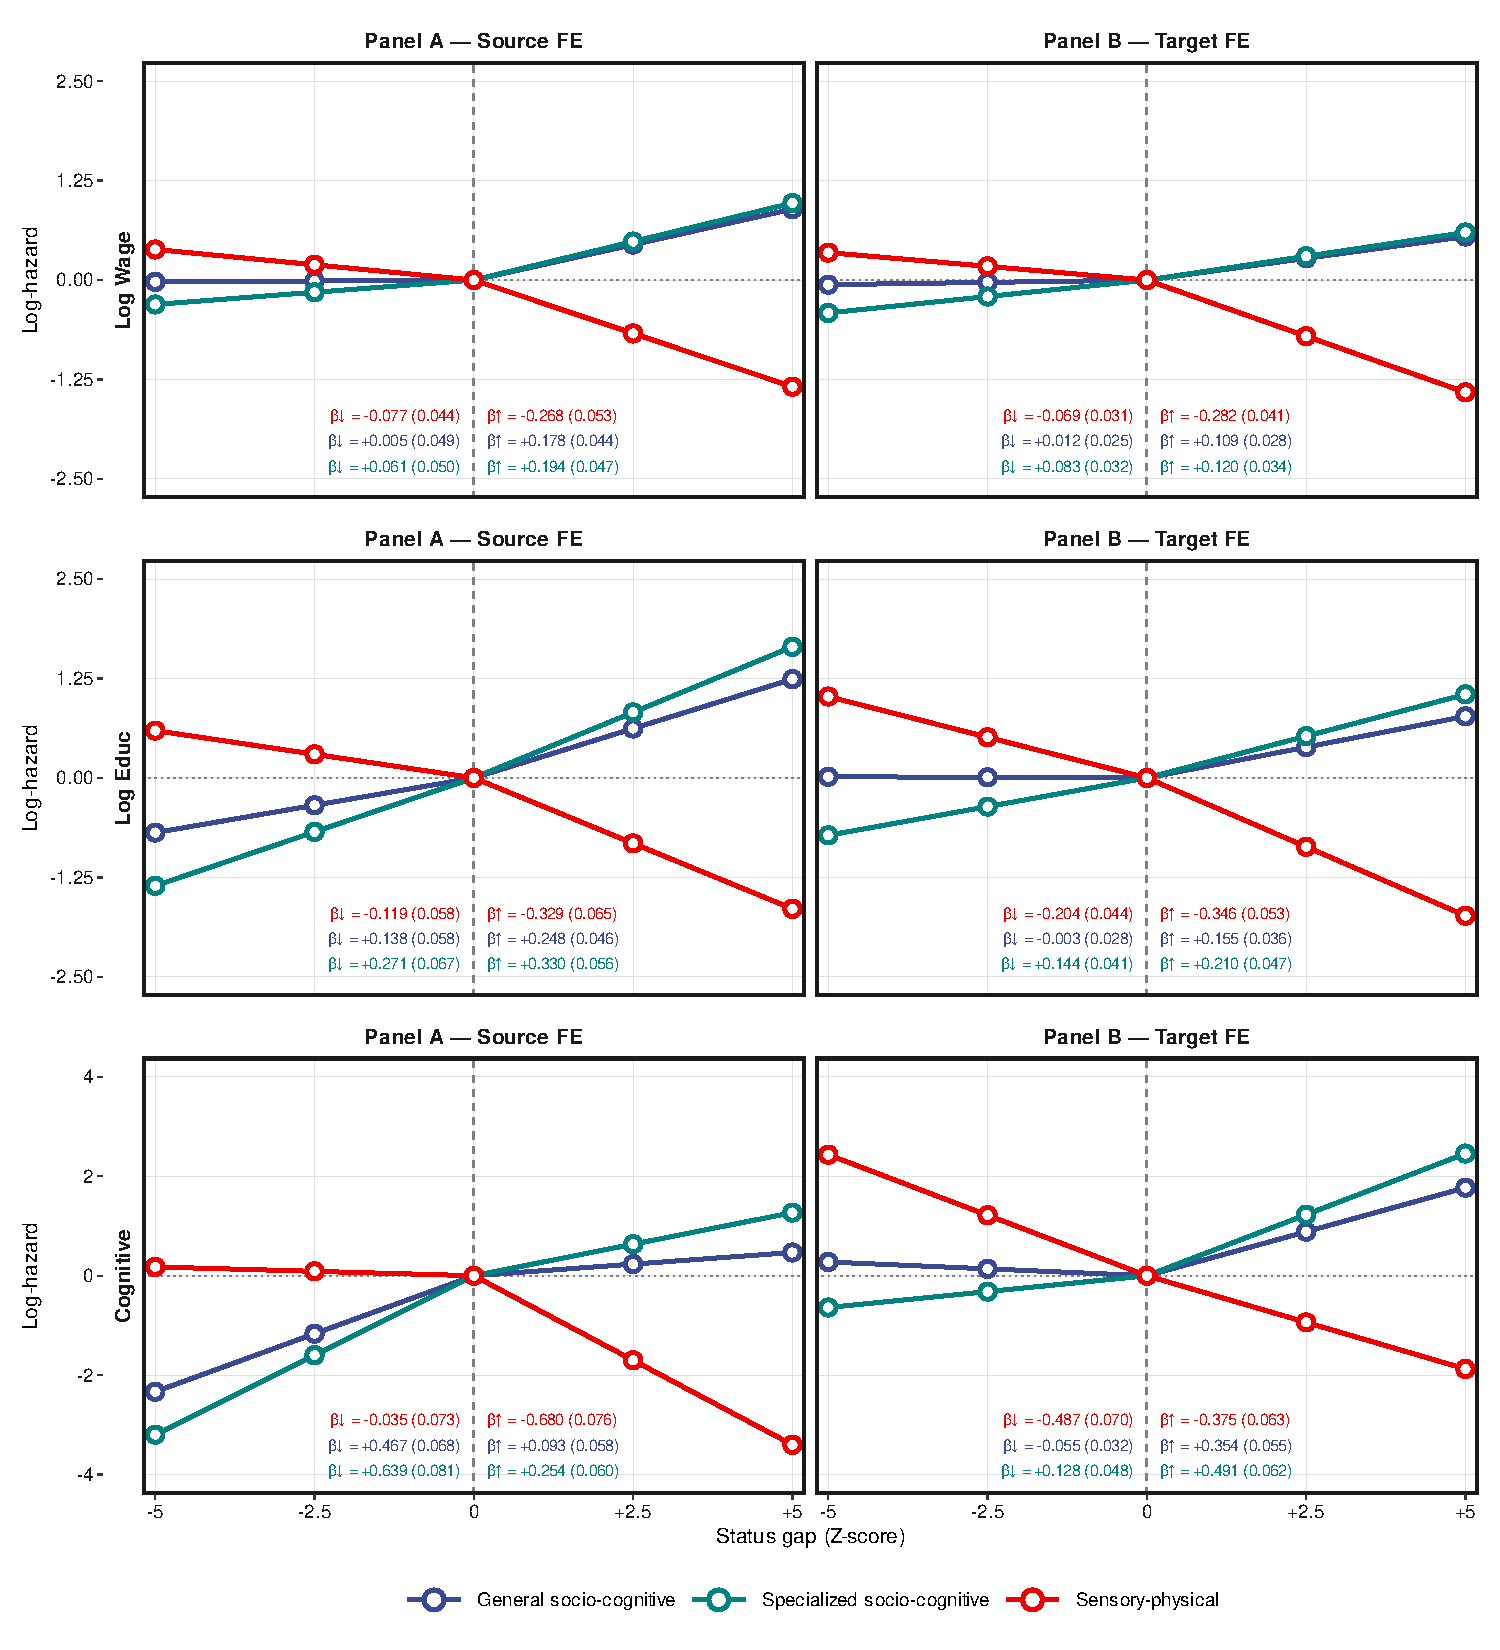
\includegraphics[width=0.8\textwidth]{figures/fig_SI_alt_status_Adoption.pdf}
    \caption{\textbf{Alternative Status Measures for Skill Adoption.} Fitted log-hazard of skill adoption as a function of the signed status gap between target and source occupations. Status gaps are computed using three alternative measures: Log wage, Log education, and Cognitive score. To ensure comparability across measures and with the main specification, all variables were standardized ($SD = 1$) at the occupation level prior to calculating the directional gaps. Panel A displays estimates controlling for source and skill fixed effects, whereas Panel B controls for target and skill fixed effects. Lines represent the estimated upward ($\beta^{\uparrow}$) and downward ($\beta^{\downarrow}$) slopes for each skill archetype. Standard errors are clustered three-way (source, target, and skill).}
    \label{fig:alt_status_adoption}
\end{figure*}
